%----------------------------------------------------------------------------------------
%	PACKAGES AND OTHER DOCUMENT CONFIGURATIONS
%----------------------------------------------------------------------------------------
\documentclass[paper=a4, fontsize=11pt]{scrartcl} % A4 paper and 11pt font size
\usepackage[T1]{fontenc} % Use 8-bit encoding that has 256 glyphs
\usepackage{fourier} % Use the Adobe Utopia font for the document - comment this line to return to the LaTeX default
\usepackage[english]{babel} % English language/hyphenation
\usepackage{amsmath,amsfonts,amsthm} % Math packages
\usepackage{lipsum} % Used for inserting dummy 'Lorem ipsum' text into the template
\usepackage{sectsty} % Allows customizing section commands
\allsectionsfont{\centering \normalfont\scshape} % Make all sections centered, the default font and small caps
\usepackage{fancyhdr} % Custom headers and footers
\usepackage[]{mcode}
\usepackage{amsmath}
\usepackage{graphics}
\usepackage{graphicx}

\pagestyle{fancyplain} % Makes all pages in the document conform to the custom headers and footers
\fancyhead{} % No page header - if you want one, create it in the same way as the footers below
\fancyfoot[L]{} % Empty left footer
\fancyfoot[C]{} % Empty center footer
\fancyfoot[R]{\thepage} % Page numbering for right footer
\renewcommand{\headrulewidth}{0pt} % Remove header underlines
\renewcommand{\footrulewidth}{0pt} % Remove footer underlines
\setlength{\headheight}{13.6pt} % Customize the height of the header

\numberwithin{equation}{section} % Number equations within sections (i.e. 1.1, 1.2, 2.1, 2.2 instead of 1, 2, 3, 4)
\numberwithin{figure}{section} % Number figures within sections (i.e. 1.1, 1.2, 2.1, 2.2 instead of 1, 2, 3, 4)
\numberwithin{table}{section} % Number tables within sections (i.e. 1.1, 1.2, 2.1, 2.2 instead of 1, 2, 3, 4)

\setlength\parindent{0pt} % Removes all indentation from paragraphs - comment this line for an assignment with lots of text

%----------------------------------------------------------------------------------------
%	TITLE SECTION
%----------------------------------------------------------------------------------------

\newcommand{\horrule}[1]{\rule{\linewidth}{#1}} % Create horizontal rule command with 1 argument of height

\title{	
\normalfont \normalsize 
\horrule{0.5pt} \\[0.4cm] % Thin top horizontal rule
\huge ECE 532 Homework 7: \\Convexity and the support vector machine\\ % The assignment title
\horrule{2pt} \\[0.5cm] % Thick bottom horizontal rule
}

\author{Qihong Lu} % Your name
\date{\normalsize\today} % Today's date or a custom date

\begin{document}

\maketitle % Print the title

%----------------------------------------------------------------------------------------
%	PROBLEM 1
%----------------------------------------------------------------------------------------

\section*{Question1 verifying convexity}

\textbf{a) Assume h and g are convex, show that f = g + h is also convex.} \\ 

Let $\alpha \in [0,1]$\\
By definition of convexity, we know that: 

\hspace{1cm} h is convex $\Rightarrow h(\alpha x_1 + (1-\alpha)x_2) \leq \alpha h(x_1) + (1-\alpha) h(x_2)$

\hspace{1cm} g is convex $\Rightarrow g(\alpha x_1 + (1-\alpha)x_2) \leq \alpha g(x_1) + (1-\alpha) g(x_2)$\\

By taking their sum, we have that 
\begin{align*}
g(\alpha x_1 + (1-\alpha)x_2) + h(\alpha x_1 + (1-\alpha)x_2) &\leq \alpha g(x_1) + (1-\alpha) g(x_2) + \alpha h(x_1) + (1-\alpha) h(x_2)	\\
g(\alpha x_1 + (1-\alpha)x_2) + h(\alpha x_1 + (1-\alpha)x_2) &\leq \alpha [g(x_1) + h(x_1)] + (1-\alpha) [g(x_2)  + h(x_2)]	\\
f(\alpha x_1 + (1-\alpha)x_2) &\leq \alpha f(x_1) + (1-\alpha) f(x_2)
\end{align*}
So f is also convex by the definition of convexity. \\\\

\newpage
\textbf{b) Show that positive quadratic form $x^TPx$ is convex, where P is p.d.}

I need to show that 
$f(\alpha x + (1-\alpha)y) \leq \alpha f(x) + (1-\alpha) f(y)$, the following inequalities are equivalent
\begin{align*}
(\alpha x + (1-\alpha)y)^T P (\alpha x + (1-\alpha)y) \leq \alpha x^T P x + (1-\alpha)y^TP y	\\
\alpha^2 x^T P  x + \alpha(1-\alpha)y^T P  x
\alpha(1-\alpha) x^T P y+ (1-\alpha)^2y^T P y
\leq \alpha x^T P x + (1-\alpha)y^TP y \\
\alpha(1-\alpha)y^T P x + \alpha(1-\alpha) x^T P y
\leq \alpha(1 - \alpha) x^T P x + \alpha(1 - \alpha)y^TP y \\
\alpha(1-\alpha)(y^T P x + x^T P y)
\leq \alpha(1 - \alpha) (x^T P x + y^TP y) \\
y^T P x + x^T P y \leq x^T P x + y^TP y \\
\end{align*}

So, to show positive quadratic form $x^TPx$ is convex, I just need to show 
$$
y^T P x + x^T P y \leq x^T P x + y^TP y
$$
Which is equavlient to 
\begin{align*}
x^T P x -  x^T P y  + y^TP y - y^T P x \geq 0	\\
x^T P (x -  y)  - y^TP (x-y) \geq 0	\\
(x^T P - y^TP )(x-y) \geq 0	\\
(x - y )^T P(x-y) \geq 0	\\
\end{align*}
And we know that $(x - y )^T P(x-y) \geq 0$ is true, because P is positive definite. 

In conclusion, positive quadratic form is convex. \\\\

\newpage
\textbf{c) show that the pointwise maximun of several affine functions: $f(x) = \underset{1 \leq i \leq m}{\max} (a_i^T x + b_i)$ are convex}\\

Let $\beta \in [0,1]$, I want to show that $f(\beta x + (1-\beta)y) \leq \beta f(x) + (1-\beta) f(y)$
\begin{align*}
f(\beta x + (1-\beta)y) &= \underset{1 \leq i \leq m}{\max} [a_i^T (\beta x + (1-\beta)y) + b_i]	\\
&= \underset{1 \leq i \leq m}{\max} [\beta a_i^T  x + (1-\beta)a_i^Ty + b_i] \\
&\leq \underset{1 \leq i \leq m}{\max} [\beta a_i^T x] + \underset{1 \leq i \leq m}{\max} [(1-\beta)a_i^Ty + b_i] \\
&= \beta \underset{1 \leq i \leq m}{\max} (a_i^T x) + (1-\beta) \underset{1 \leq i \leq m}{\max} (a_i^Ty + \frac{b_i}{1-\beta} ) \\
\end{align*}
These two terms can be bounded individually, that in particular:  
\begin{align*}
\beta \underset{1 \leq i \leq m}{\max} (a_i^T x) \leq \beta \underset{1 \leq i \leq m}{\max} (a_i^T x + b_i) \\
(1-\beta) \underset{1 \leq i \leq m}{\max} (a_i^Ty + \frac{b_i}{1-\beta} ) \leq (1-\beta) \underset{1 \leq i \leq m}{\max} (a_i^T y + b_i)
\end{align*}
Therefore we have that 
\begin{align*}
\beta \underset{1 \leq i \leq m}{\max} (a_i^T x) + (1-\beta) \underset{1 \leq i \leq m}{\max} (a_i^Ty + \frac{b_i}{1-\beta} ) &\leq \beta \underset{1 \leq i \leq m}{\max} (a_i^T x + b_i) + (1-\beta) \underset{1 \leq i \leq m}{\max} (a_i^T y + b_i)	\\
\Rightarrow \beta \underset{1 \leq i \leq m}{\max} (a_i^T x) + (1-\beta) \underset{1 \leq i \leq m}{\max} (a_i^Ty + \frac{b_i}{1-\beta} ) &\leq \beta f(x) + (1-\beta) f(y) \\
\Rightarrow f(\beta x + (1-\beta)y) \leq \beta f(x) + (1-\beta) f(y)
\end{align*}

In conclusion, $f(x) = \underset{1 \leq i \leq m}{\max} (a_i^T x + b_i)$ are convex. 

\newpage
\textbf{d) An matrix function example. $f: \mathbb{R}^{mxn} \rightarrow \mathbb{R}$. Show that $f(X) = \|X\|_2$, the induced 2 norm is convex}\\


Let $A \in \mathbb{R}^{mxn}, B \in \mathbb{R}^{mxn}, \beta \in [0,1]$. 

I need to show that $f(\beta A + (1-\beta)B) \leq \beta f(A) + (1-\beta) f(B)$, which is the same as: 


By the triangle inequality 
\begin{align*}
\text{LHS} = \|\beta A + (1-\beta)B \| \leq \|\beta A \| + \| (1-\beta)B \| = \beta \|A\| + (1-\beta) \|B\| = \text{RHS}
\end{align*}
This tells us that 
$$ \|\beta A + (1-\beta)B \| \leq \beta \|A\| + (1-\beta) \|B\| $$

Therefore the induced matrix 2 norm is convex. 


%----------------------------------------------------------------------------------------
%	PROBLEM 2
%----------------------------------------------------------------------------------------
\newpage
\section*{Question2 Gradient decent \& Stochastic Gradient decent}


\textbf{a) generate the data with different noise}\\
\textbf{b) Implement GD and SGD to solve the l1 loss and compare it with LS}

My answers for question a and b are combined here:

\begin{center}
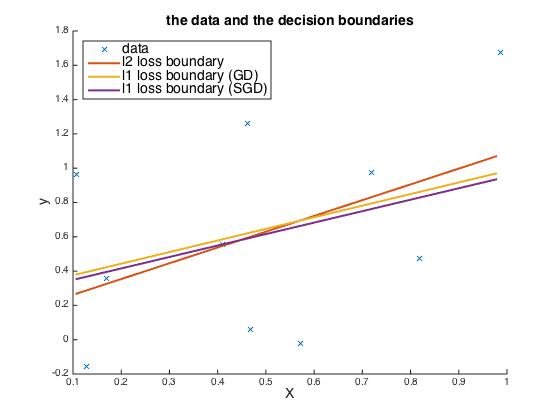
\includegraphics[scale=.5]{hw7_2a_fit.jpg}
\end{center}
\begin{center}
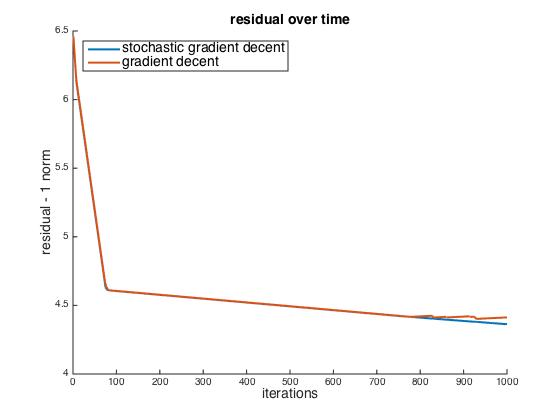
\includegraphics[scale=.5]{hw7_2a_gdsgd.jpg}
\end{center}

Here, the error component is standard normal. The standard least square and L1 loss found very similar fits. The solutions provided by gradient decent and stochastic gradient decent are often very similar. It does seem that gradient decent is not as stable as stochastic decent. 

\newpage
Simulation with smaller error 
\begin{center}
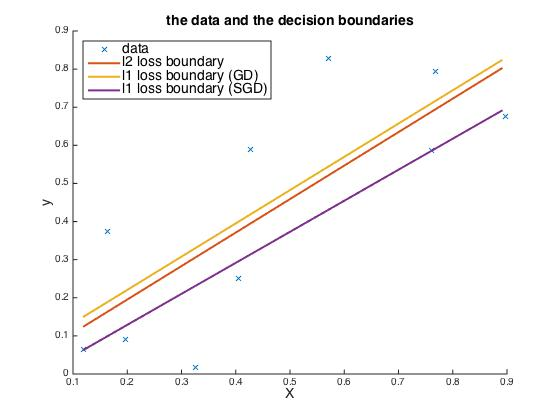
\includegraphics[scale=.5]{hw7_2a_smer_fit.jpg}
\end{center}
\begin{center}
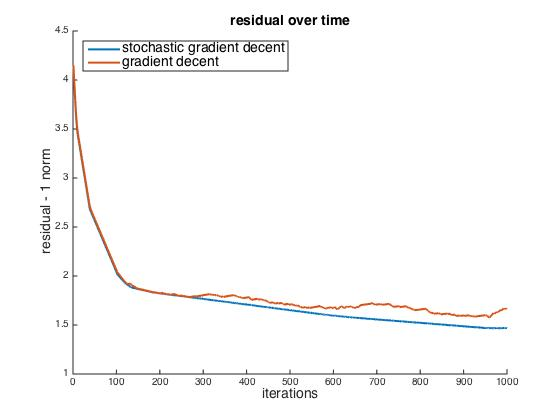
\includegraphics[scale=.5]{hw7_2a_smer_gdsgd.jpg}
\end{center}

Here, the error component generated standard normal and divided by 5, so the error magnitude is smaller than previous simulation. Again, the standard least square and L1 loss found very similar fits. Consistenly with the previous simulation, stochastic gradient decent seems to be more stable than gradient decent on reducing the residual over time

\newpage
\textbf{c) laplacian noise}
\begin{center}
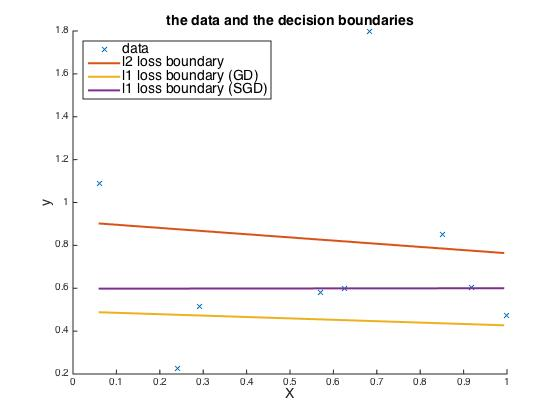
\includegraphics[scale=.5]{hw7_2c_fit.jpg}
\end{center}
\begin{center}
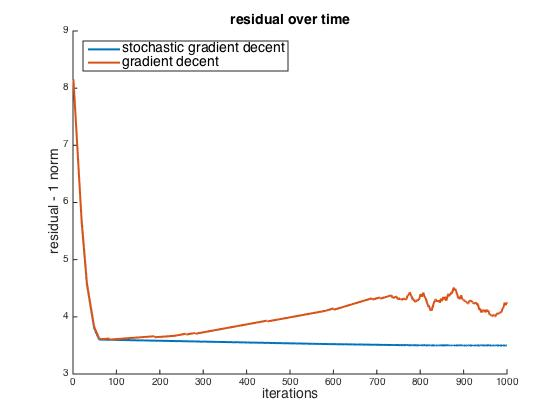
\includegraphics[scale=.5]{hw7_2c_gdsgd.jpg}
\end{center}

Again, when using laplacian noise, we still see stochastic gradient decent seems to be able to converged at a better weight configuration over time. Additionaly, from this plot, I realized that l2 loss, or the least square optimization seems to be more sensitive to outlier point. Here, it seems that the least square  fit is pulled by the outlier point on the top. The reason why least square is more sensitive to farther point is that the loss function is squaring the deviation, so point with large deviation would be magnified. 

\newpage
Simulation with smaller error 
\begin{center}
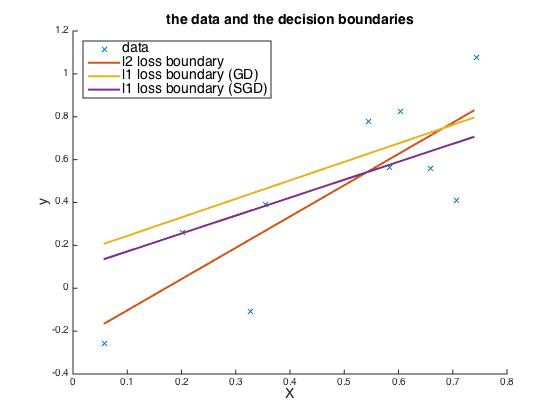
\includegraphics[scale=.5]{hw7_2c_smer_fit.jpg}
\end{center}
\begin{center}
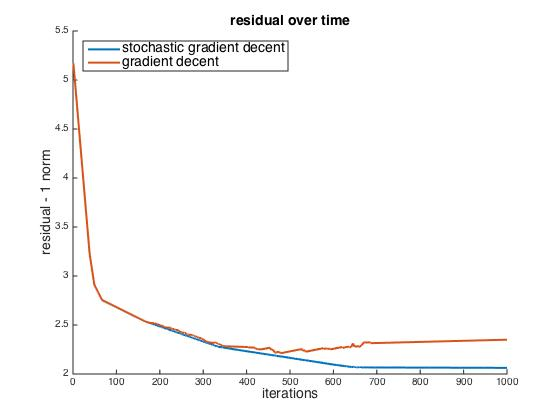
\includegraphics[scale=.5]{hw7_2c_smer_gdsgd.jpg}
\end{center}

Overall, gradient decent and stochastic gradient decent give rise to similar results. However, stochastic gradient decent still converged to a better weight configuration over time. And similar to the previous simulation, it seems that least square method is more sensitive to farther points. 

\newpage
Matlab code for question 2: 
\begin{lstlisting}
%% initialization - simulation parameters
close all; clear; clc;
m = 10;     % num data points
w.true = [0 ;1];
lapNoise = 1; 


%% simulate the data
% generate data X ~ unif[0,1]
x = unifrnd(0,1,m,1);
x = [ones(m,1) x];
% Gaussian noise
if ~lapNoise
    err = randn(m,1)/5;
else 
    err = laprnd(m,1)/5;
end
% then generate y
y = x * w.true + err;

%% LS fit
w.ls = inv(x' * x) * x' * y;


%% l1 loss - gradient decent 
% set learning rate 
tau = 0.001;

% preallocate 
numIters = 1000;
w.gd = zeros(size(w.true));
w.sgd = zeros(size(w.true));
residual.sgd = nan(numIters,1);
% iterative alg.
for j = 1 : numIters
    %% random permutation stochastic decent procedure
    for i = randperm(m)
        % compute the stochastic gradient for 1 training example 
        if (y(i) - x(i,:) * w.sgd) > 0
            sgd = x(i,:)';
        elseif (y(i) - x(i,:) * w.sgd) < 0
            sgd = -x(i,:)';
        else
            sgd = zeros(size(w.true));  % sub grad
        end
        % stochastic gradient decent update
        w.sgd = w.sgd + tau * sgd;
    end
    
    
    %% gradient decent procedure
    gd = zeros(size(w.true));
    for i = 1:m
        % compute the gradient for 1 training example 
        if (y(i) - x(i,:) * w.sgd) > 0
            sgd = x(i,:)';
        elseif (y(i) - x(i,:) * w.sgd) < 0
            sgd = -x(i,:)';
        else
            sgd = zeros(size(w.true));  % sub grad
        end
        % accumulate gradients 
        gd = gd + sgd;
    end
    % gradient decent update
    w.gd = w.gd + tau * gd;
    
    %% record the residual
    residual.sgd(j) = norm(y - x * w.sgd,1);
    residual.gd(j) = norm(y - x * w.gd,1);
end


%%
[w.true w.ls w.sgd w.gd]

%% plot the data and decision boundary
hold on 
plot(x(:,2), y, 'x')
boundary.x = min(x(:,2)) :0.01: max(x(:,2));
boundary.y.ls = w.ls(1) + w.ls(2) * boundary.x;
boundary.y.gd = w.gd(1) + w.gd(2) * boundary.x;
boundary.y.sgd = w.sgd(1) + w.sgd(2) * boundary.x;
plot(boundary.x, boundary.y.ls, 'linewidth', 2)
plot(boundary.x, boundary.y.gd, 'linewidth', 2)
plot(boundary.x, boundary.y.sgd, 'linewidth', 2)
hold off

% add some text 
FS = 14; 
xlabel('X','fontsize', FS)
ylabel('y','fontsize', FS)
title('the data and the decision boundaries','fontsize', FS)
legend({'data', 'l2 loss boundary', 'l1 loss boundary (GD)', 'l1 loss boundary (SGD)'},'fontsize', FS, 'location', 'northwest')

%% plot residual over time 
figure
hold on 
plot(residual.sgd, 'linewidth', 2)
plot(residual.gd', 'linewidth', 2)
hold off
legend({'stochastic gradient decent', 'gradient decent'},'fontsize', FS, 'location', 'northwest')
xlabel('iterations','fontsize', FS)
ylabel('residual - 1 norm','fontsize', FS)
title('residual over time','fontsize', FS)
\end{lstlisting}

%----------------------------------------------------------------------------------------
%	PROBLEM 3
%----------------------------------------------------------------------------------------
\newpage
\section*{Question3 Error Bounds using Hinge Loss}
Consider the using stochastic gradient decent to solve the hinge loss optimization: 

$$\underset{w}{\min} \sum_{i=1}^{m} (1 - y_i x_i^T w)_+ $$ \\ 
\textbf{a) derive a boud on the average error. Assume $w_1 = 0, \|w^* \| \leq 1, \|x_i \| \leq 1, \tau = \frac{1}{\sqrt{T}} $ }

(To make sure I can understand what I wrote later, the begining the following statements is redundant with the notes.)

\begin{align*}
\| w_{t+1} - w^* \|_2^2 & = \| w_{t} - \tau \bigtriangledown f_t(w_t) - w^* \|_2^2	\\
&= \| (w_{t} - w^*) - \tau \bigtriangledown f_t(w_t)  \|_2^2		\\
&= \|w_{t} - w^*\|_2^2 + \tau^2 \| \bigtriangledown f_t(w_t)  \|_2^2	 - 2 \tau \bigtriangledown f_t(w_t)^T (w_{t} - w^*)	\\
\end{align*}

By rearragind the term, we have that 
\begin{align*}
2 \tau \bigtriangledown f_t(w_t)^T (w_{t} - w^*) = 
\| w_{t} - w^*\|_2^2 - \| w_{t+1} - w^* \|_2^2 + \tau^2 \| \bigtriangledown f_t(w_t) \|_2^2	\\
\Rightarrow
\bigtriangledown f_t(w_t)^T (w_{t} - w^*) = \frac{\| w_{t} - w^*\|_2^2 - \| w_{t+1} - w^* \|_2^2}{2 \tau } + \frac{ \tau  \| \bigtriangledown f_t(w_t) \|_2^2}{2}
\end{align*}

By convexity, the left hand side can be bounded: 
$$
\bigtriangledown f_t(w_t)^T (w_{t} - w^*) \leq f(w_{t}) - f(w^*) 
$$

Apply this bound to the equation, we get that 
$$
f(w_{t}) - f(w^*) 
\leq 
\frac{\|w_{t} - w^*\|_2^2 - \| w_{t+1} - w^* \|_2^2}{2 \tau } + \frac{ \tau  \| \bigtriangledown f_t(w_t) \|_2^2}{2}	\\
$$

The equality would holds when taking the sum of both sides from 1 to T. 
$$
\frac{1}{T} \sum_{t=1}^{T} f(w_{t}) - f(w^*) 
\leq 
\frac{1}{T} \sum_{t=1}^{T} \Big(\frac{\| w_{t} - w^*\|_2^2}{2 \tau } -  \frac{\| w_{t+1} - w^* \|_2^2}{2 \tau }
+ \frac{ \tau  \| \bigtriangledown f_t(w_t) \|_2^2}{2} \Big)	
$$
$$
\frac{1}{T} \sum_{t=1}^{T} f(w_{t}) - f(w^*) 
\leq 
\frac{\| w_1 - w^*\|_2^2}{2 \tau T}
+ \frac{ \tau }{2} \| \bigtriangledown f_t(w_t) \|_2^2
$$

By the assumptions, $w_1 = 0, \|w^*\| \leq 1$, so $\| w_1 - w^*\|_2^2 = \|-w^*\| \leq 1$. Also, $\tau = \frac{1}{\sqrt{T}}$. Therefore,

$$
\frac{1}{T} \sum_{t=1}^{T} f(w_{t}) - f(w^*) 
\leq \frac{1}{2 \sqrt{T}} + \frac{1}{2 \sqrt{T}} \| \bigtriangledown f_t(w_t) \|_2^2
$$\\

So I need a bound for $\| \bigtriangledown f_t(w_t) \|_2^2$. 

$$
f_i(w_t) = (1 - y_i x_i^T w)_+
$$

The gradient is 
\[
\bigtriangledown f_i(w_t) = 
\begin{cases}
0 				& \text{if } 1 - y_i x_i^T w \leq 0 \\
-y_i x_i          & \text{if } 1 - y_i x_i^T w > 0 
\end{cases}
\]

By the property of the norm, $\| 0 \| = 0 $, which is smaller than $\|y_i x_i\|$. So I need to bound $\|y_i x_i\|$. By the assumption, $\|x_i\| \leq 1 $ and since $y = {+1, -1}$, we have that $y_i x_i \leq 1 $. It follows that $\|y_i x_i\| \leq 1 $. \\
Therefore, 
$$
\|y_i x_i\|_2^2 = \| \bigtriangledown f_t(w_t) \|_2^2 \leq 1
$$

Go back to the average error, we have that 
\begin{align*}
\frac{1}{T} \sum_{t=1}^{T} f(w_{t}) - f(w^*) 
& \leq \frac{1}{2 \sqrt{T}} + \frac{1}{2 \sqrt{T}} 1	\\
\frac{1}{T} \sum_{t=1}^{T} f(w_{t}) - f(w^*) 
& \leq \frac{1}{\sqrt{T}}
\end{align*}

To summarize, under everything we assumed, the bound for the average error is $\frac{1}{\sqrt{T}}$.\\\\\\

\textbf{b) How many iterations are required to guarantee that the average error is less than 0.01?}\\

I can use the bound derived previously so solve for the number of iterations needed:  
\begin{align*}
\frac{1}{\sqrt{T}} & \leq \frac{1}{100}	\\
\Rightarrow \sqrt{T} & \geq 100	\\
\Rightarrow T & \geq 10000
\end{align*}

So under everything I assumed, error smaller than 0.01 can be guaranted after 10000 iterations. 

%----------------------------------------------------------------------------------------
%	PROBLEM 4
%----------------------------------------------------------------------------------------
\newpage
\section*{Question4 Classification and the SVM}

\textbf{a) reporduce the graph and plot the LS boundary}
\begin{center}
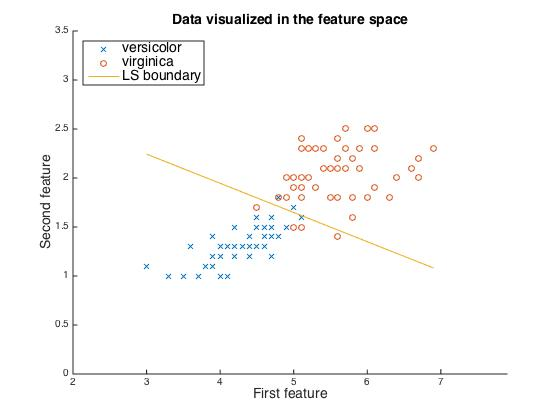
\includegraphics[scale=.6]{hw7_4a_532.jpg}
\end{center}

Here's the plot replicating the graph given in the homework. The yellow line is the decision boundary for the standard least square fit.

\newpage
\textbf{b) plot the SVM boundary}\\
Parameters:
$\lambda = 0.1, \tau = 0.003, T = 20,000, w_0 = 0$
\begin{center}
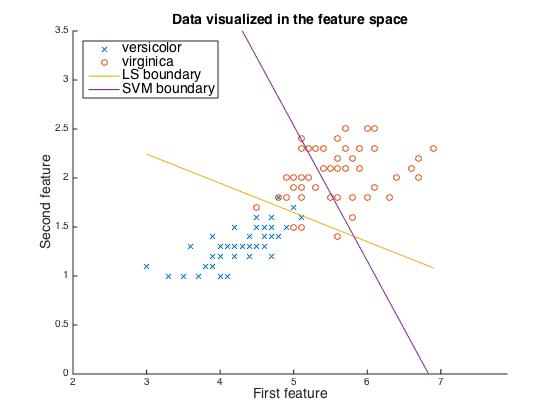
\includegraphics[scale=.6]{hw7_4b_532.jpg}
\end{center}

\begin{center}
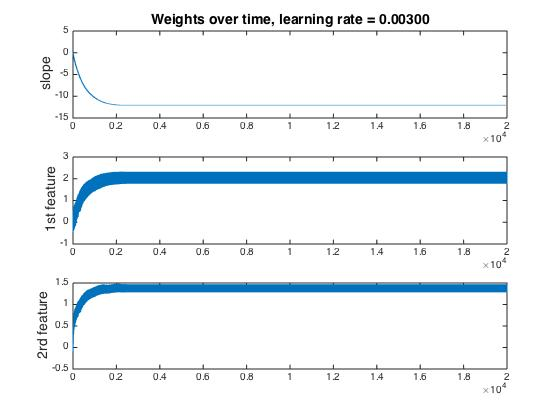
\includegraphics[scale=.5]{hw7_4b_weights_532.jpg}
\end{center}

The svm classifier performed worse than the least square classifer, in the sense that the number of misclassified examples is higher. However, the main reason is that the learning rate for the svm is too large here. This can be seen by plotting the weights over time, the second and the third weights were oscillating and did not converge at the very end. 


\newpage
\textbf{c) Compare different learning rate}\\
Small learning rate: Parameters:
$\lambda = 0.1, \tau = 0.0001, T = 20,000, w_0 = 0$
\begin{center}
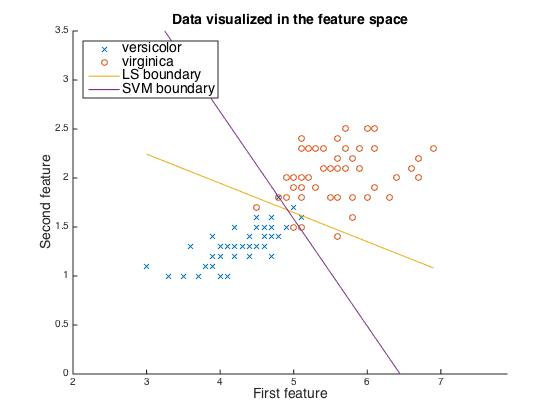
\includegraphics[scale=.6]{hw7_4c_smlr_532.jpg}
\end{center}
\begin{center}
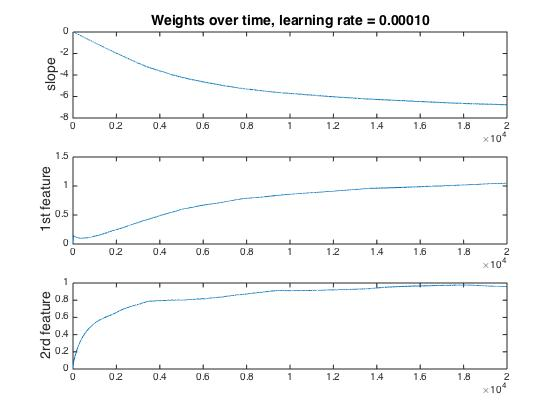
\includegraphics[scale=.5]{hw7_4c_smlr_weights_532.jpg}
\end{center}

When using a smaller learning rate, the SVM boundary looks much more reasonable. And the performance of the SVM classifer is better than the LS in this case, since it has less misclassified examples. The plots that visualize weights change over time look much smoother. At the end, all the weights converged, in the sense that no weight is having big change. 

\newpage
Larger learning rate: Parameters:
$\lambda = 0.1, \tau = 0.1, T = 20,000, w_0 = 0$
\begin{center}
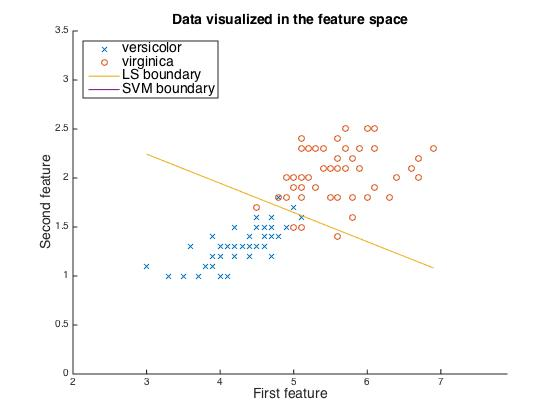
\includegraphics[scale=.6]{hw7_4c_biglr_532.jpg}
\end{center}
\begin{center}
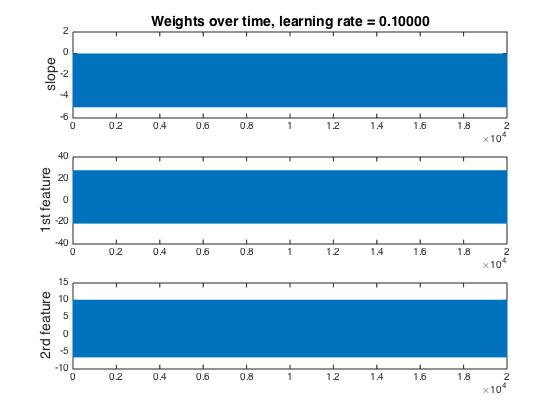
\includegraphics[scale=.5]{hw7_4c_biglr_weights_532.jpg}
\end{center}

When using a big learning rate, the plots that visualize weights change over time look terrible. All the weights are oscillating and never converged. Also, the decision boundary is bad. Indeed, it is not even on the plot. 


\newpage
Matlab code for question 4: 
\begin{lstlisting}
%% ECE 532 - HW7
clear all;clc;close all;
% initialization
load fisheriris.mat

% some parameters
numData = 50;
% no feature selection & no projection
X = meas(51:end,3:4);
X = [ones(100,1), X];
% versicolor = -1
% virginica  = 1
y = [-1* ones(numData,1); ones(numData,1)];

%% plot the data
hold on
plot(X(y ==-1,2), X(y ==-1,3), 'x')
plot(X(y == 1,2), X(y == 1,3), 'o')


FS = 14;
xlim([min(X(:,2))-1 max(X(:,2))+1])
ylim([min(X(:,3))-1 max(X(:,3))+1])
title('Data visualized in the feature space', 'fontsize', FS)
xlabel('First feature', 'fontsize', FS)
ylabel('Second feature', 'fontsize', FS)


%% fit standard ls
w.ls = inv(X' * X) * X' * y;

% plot the decision boundary for ls.
boundary.f1_range = [min(X(:,2)) :0.01: max(X(:,2))];
boundary.f2_val.ls = -w.ls(1)/w.ls(3)-(w.ls(2)/w.ls(3)) .* boundary.f1_range';
plot(boundary.f1_range, boundary.f2_val.ls);
% legend({'versicolor', 'virginica', 'LS boundary'}, 'fontsize', FS, 'location', 'northwest')

%% fit svm
tau = 0.003;
lambda = .1;
w.svm = zeros(size(X,2),1);
numIters = 20000;
record.svmw = nan(length(w.svm),numIters);
% implement gradient decent
for i = 1 : numIters
    
    change = zeros(3,1);
    % accumulate the gradient for all training examples
    for j = 1 : length(y)
        if y(j) * X(j,:) * w.svm < 1
            change(1) = change(1) - tau * y(j) * X(j,1)';
            change(2:3) = change(2:3) - tau*(y(j) * X(j,2:3)' - 2*lambda * w.svm(2:3));
        end
    end
%     change(2:3) 
    
    % gradient decent update
    w.svm = w.svm - change;
    % save weights
    record.svmw(:,i) = w.svm;
    % 
    disp(i)
    norm(y - X * w.svm)
end

%% plot svm boundaries
boundary.f2_val.svm = -w.svm(1)/w.svm(3)-(w.svm(2)/w.svm(3)) .* boundary.f1_range';
plot(boundary.f1_range, boundary.f2_val.svm)
legend({'versicolor', 'virginica','LS boundary', 'SVM boundary'},'fontsize', FS, 'location', 'northwest')
hold off
%% plot weights
figure
subplot(3,1,1)
plot(record.svmw(1,:))
title_text = sprintf('Weights over time, learning rate = %.5f', tau);
title(title_text,'fontsize', FS)
ylabel('slope','fontsize', FS)
subplot(3,1,2)
plot(record.svmw(2,:))
ylabel('1st feature','fontsize', FS)
subplot(3,1,3)
plot(record.svmw(3,:))
ylabel('2rd feature','fontsize', FS)

\end{lstlisting}

\end{document}